\subsection{Login}
I dette afsnit vises design, brugergrænseflade, implementering og test for 'Login' viewet. For den fulde dokumentation henvises til Arkitektur og Design dokumentationens afsnit \ref{Design-sec:Login}.
\subsubsection{Design}
Sekvensdiagrammet for 'Login' viewet til Rambøll Tilsyn, kan ses på Figur \ref{fig:LoginSekvens}. Figuren viser det logiske flow, der sker når brugeren vil logge ind.
\begin{figure}[H] % (alternativt [H])
	\centering
	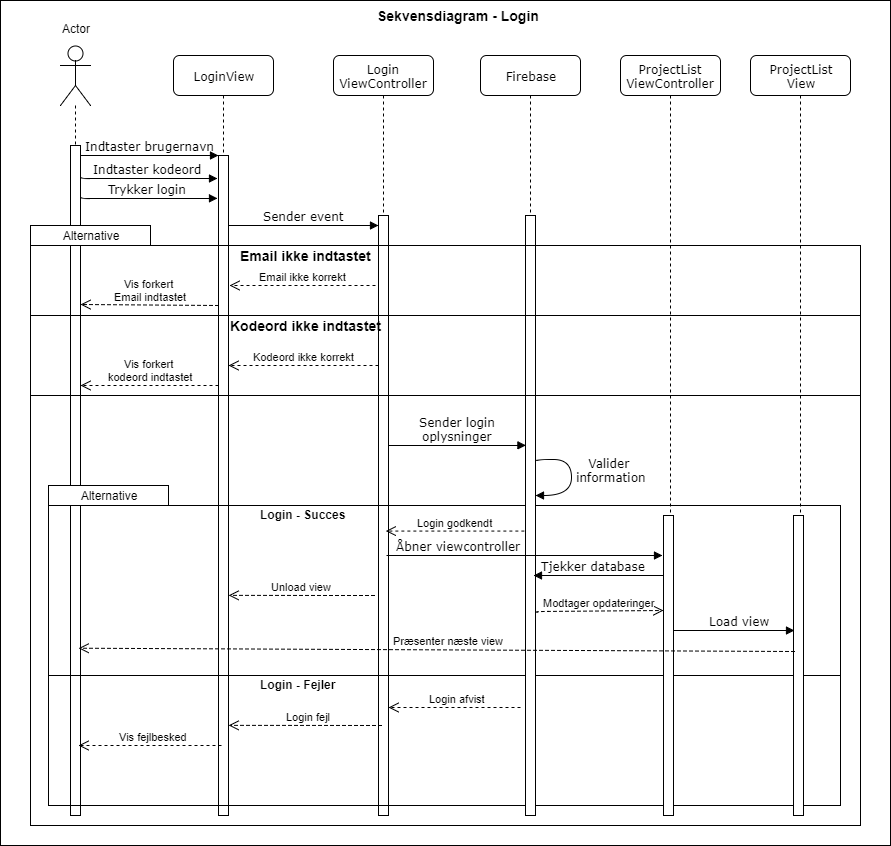
\includegraphics[height=15cm, width=15cm]{Design/Applikation/Login/LoginSekvensDiagram}
	\caption{Sekvensdiagram for Login i Rambøll Tilsyn.}
	\label{fig:LoginSekvens}
\end{figure}

\clearpage

\subsubsection{Grafisk brugergrænseflade}
Den grafiske brugergrænseflade for 'Login' viewet består af felter til at brugeren kan indtaster sit brugernavn og kodeord. Se Figur \ref{fig:LoginView}
\begin{figure}[H] % (alternativt [H])
	\centering
	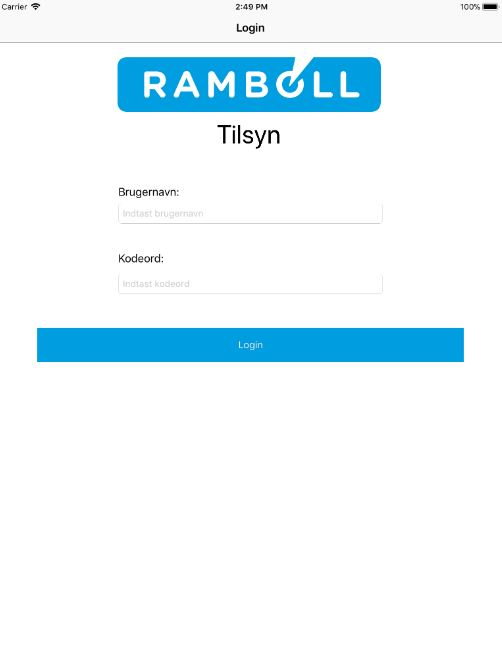
\includegraphics[height=12cm, width=10cm]{Design/Applikation/Login/LoginView}
	\caption{Login viewet som det er implementeret i Rambøll Tilsyn.}
	\label{fig:LoginView}
\end{figure}

\subsubsection{Implementering}
Når applikationen åbner og login siden kommer frem, starter Firebase med at kontrollerer om der allerede er en bruger som er logget ind. Er der en bruger logget ind, navigeres man direkte videre til 'Project List' viewet. Hvis ikke der er en bruger logget ind, skal brugeren logge ind, for at kunne benytte applikationen. \\
Når login bliver loadet, sættes der en eventhandler på login knappen, så når bruger trykker på den, vil der blive forsøgt at logge ind på applikationen. \\
Der bliver også indsat placeholders i tekstfelterne for e-mail og kodeord. Når brugeren begynder at skrive kodeord, vil dette være masked, så kodeordet ikke står i klar tekst. \\
Når brugeren trykker på login, sendes værdierne fra tekstfelterne til Firebase, som her validerer oplysningerne. Er oplysningerne korrekte, vil brugeren blive navigeret til 'Project List' viewet. Hvis de er forkerte, vil der blive vist en fejlmeddelelse til brugeren. \\
For en mere deltajeret beskrivelse af implementeringen og kode snips, henvises til Arkitektur og Design dokumentations afsnit \ref{Design-sec:Login}.

\clearpage